\documentclass[a5paper]{article}

\usepackage{chirpstyle}
\usepackage{tikz}

\begin{document}

\section*{Geometric Probability: Line Segments Form a Triangle}

\begin{chirpbox}
    \begin{problem}
        Take a line segment of length \( 1 \) and randomly divide it into three
        segments. What is the probability that these lengths form a valid
        (possibly degenerate) triangle?
    \end{problem}
\end{chirpbox}

\begin{figure}[h!]
    \centering
    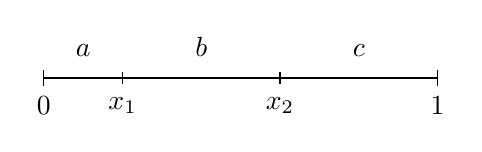
\begin{tikzpicture}[scale=5]
        \draw (0, 0) -- (1, 0);
        \draw (0, -0.02) -- (0, 0.02);
        \draw (1, -0.02) -- (1, 0.02);

        \node at (0, -0.07) {\( 0 \)};
        \node at (1, -0.07) {\( 1 \)};

        \draw (0.2, -0.015) -- (0.2, 0.015);
        \draw (0.6, -0.015) -- (0.6, 0.015);
        \node at (0.2, -0.07) {\( x_1 \)};
        \node at (0.6, -0.07) {\( x_2 \)};

        \node at (0.1, 0.07) {\( a \)};
        \node at (0.4, 0.08) {\( b \)};
        \node at (0.8, 0.07) {\( c \)};
    \end{tikzpicture}
    \caption{Geometric intuition for how we define our side lengths.}
\end{figure}

\begin{solution}
    We claim that the probability is \( 1/4 \). This can obtained with just a
    little bit of working with random variables.

    Let \( x_1, x_2 \) be identical, independent random variables distributed
    over \( \textsf{Uniform}(0, 1) \). Consider the case when \( x_2 > x_1 \).
    (the complement case is equally likely so we shall double our final
    probability answer to account for this) We may form the lengths of our
    triangle \( a, b, c \) as follows (refer to the Figure 1 for geometric
    intuition):
    \[
        a := x_1, \quad b := x_2 - x_1, \quad c := 1 - x_2
    .\]
    We can now use all cycles of the triangle inequality to get bounds for
    these random variables.
    \begin{align*}
        \textcolor{Cerulean}{C_1}: a &\le b + c \implies x_1 \le 1/2, \\
        \textcolor{WildStrawberry}{C_2}: b &\le a + c \implies x_2 \le x_1 + 1/2, \\
        \textcolor{Yellow}{C_3}: c &\le a + b \implies x_2 \ge 1/2
    .\end{align*}
    We may graph these inequalities in the unit square to get our desired area (refer to Figure 2). Doing so, we see that the area of the triangle is \( 1/8 \). Doubling this because of symmetry, we arrive at an answer of \( \boxed{1/4} \).
\end{solution}

\begin{figure}
    \centering
    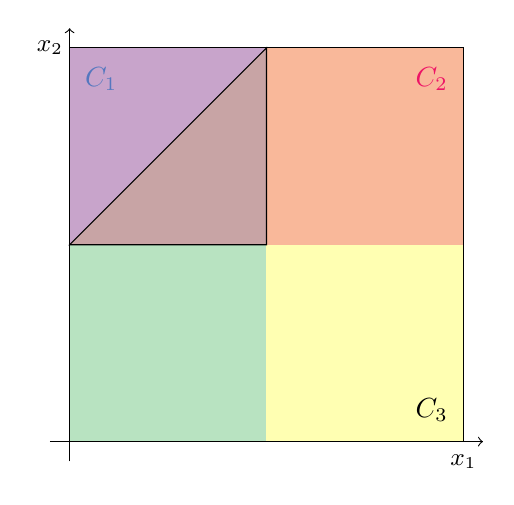
\begin{tikzpicture}[scale=5]
        \fill[Yellow, opacity=0.3] (0, 0.5) -- (0.5, 1) -- (1, 1) -- (1, 0) -- (0, 0) -- cycle;
        \node[Black] at (0.92, 0.08) {\( C_3 \)};

        \fill[Cerulean, opacity=0.3] (0, 0) -- (0, 1) -- (0.5, 1) -- (0.5, 0) -- cycle;
        \node[Cerulean] at (0.08, 0.92) {\( C_1 \)};

        \fill[WildStrawberry, opacity=0.3] (0, 0.5) -- (0, 1) -- (1, 1) -- (1, 0.5) -- cycle;
        \node[WildStrawberry] at (0.92, 0.92) {\( C_2 \)};

        \draw (0, 0.5) -- (0.5, 1) -- (0.5, 0.5) -- cycle;

        \draw[->] (-0.05, 0) -- (1.05, 0);
        \draw[->] (0, -0.05) -- (0, 1.05);

        \node at (-0.05, 1) {\small \( x_2 \)};
        \node at (1, -0.05) {\small \( x_1 \)};

        \draw (0, 1) -- (1, 1) -- (1, 0);
    \end{tikzpicture}
    \caption{A graph of the three conditions from triangle inequality.}
\end{figure}

\begin{remark}
    The cases where the triangle is degenerate have measure \( 0 \), so this
    problem is the exact same if you rule out degeneracies.
\end{remark}

\begin{remark}
    One must be careful in how they decide to randomly pick the line segment
    lengths. One may try to go about generating lengths through normalization, like so:
    \[
        a = \frac{x_1}{x_1 + x_2 + x_3}, \quad b = \frac{x_2}{x_1 + x_2 + x_3}, \quad c = \frac{x_3}{x_1 + x_2 + x_3}
    ,\]
    however this will land you into deep trouble because these lengths are not uniformly distributed at all!
\end{remark}

I'm not so certain that this problem even generalizes to higher dimensions, but
it may be something to revisit.

\end{document}
